\providecommand{\main}{../../../..}
\documentclass[\main/dresen_thesis.tex]{subfiles}
\begin{document}
  \label{sec:colloidalCrystals:vsm}

  \begin{figure}[tb]
    \centering
    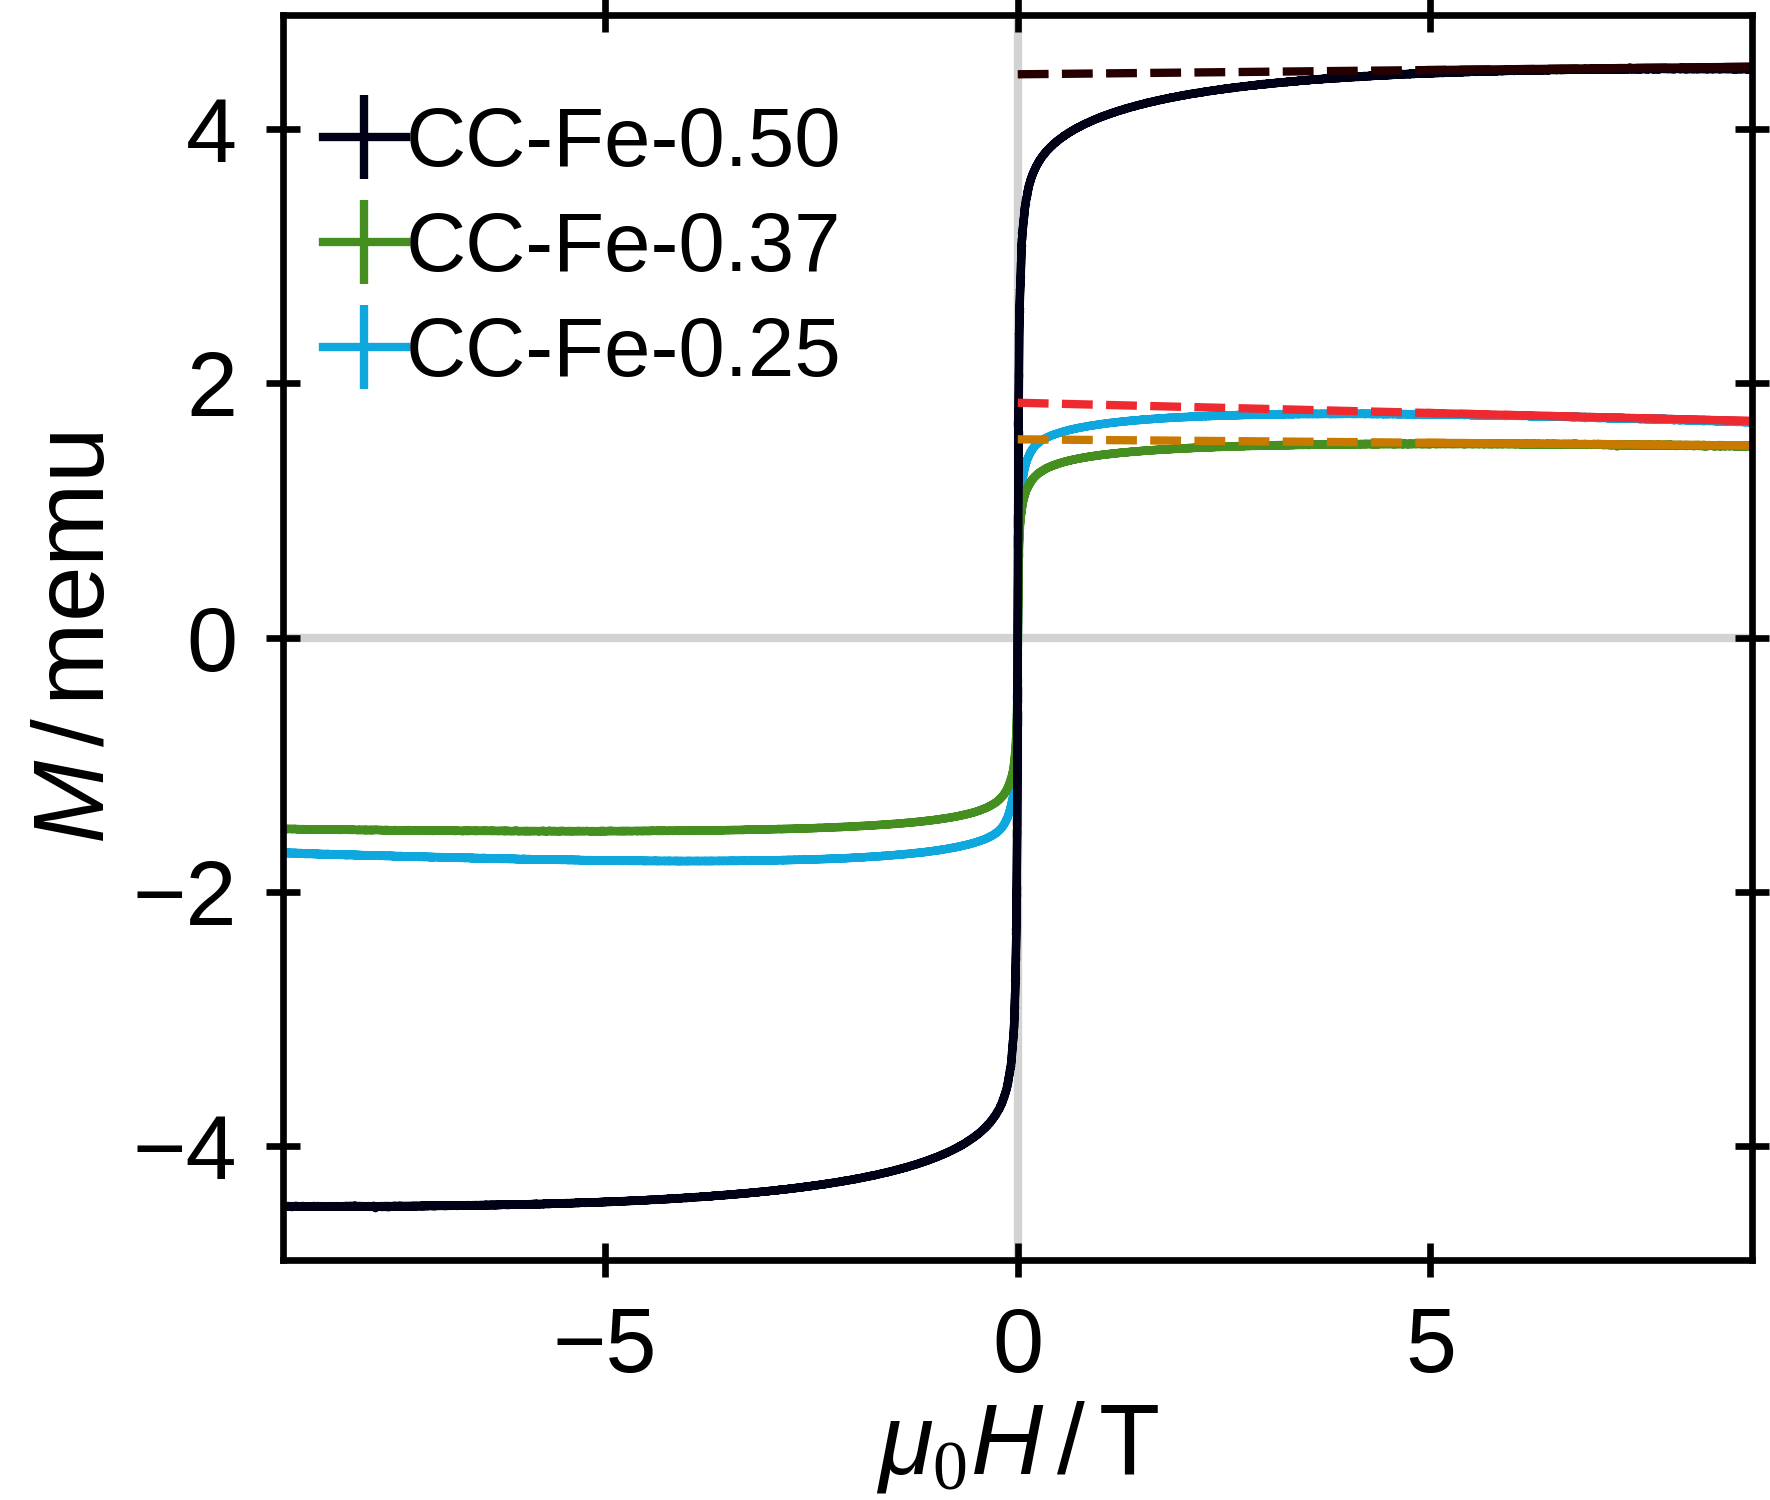
\includegraphics{colloidalCrystals_PPMS_300KrawData_allSamples}
    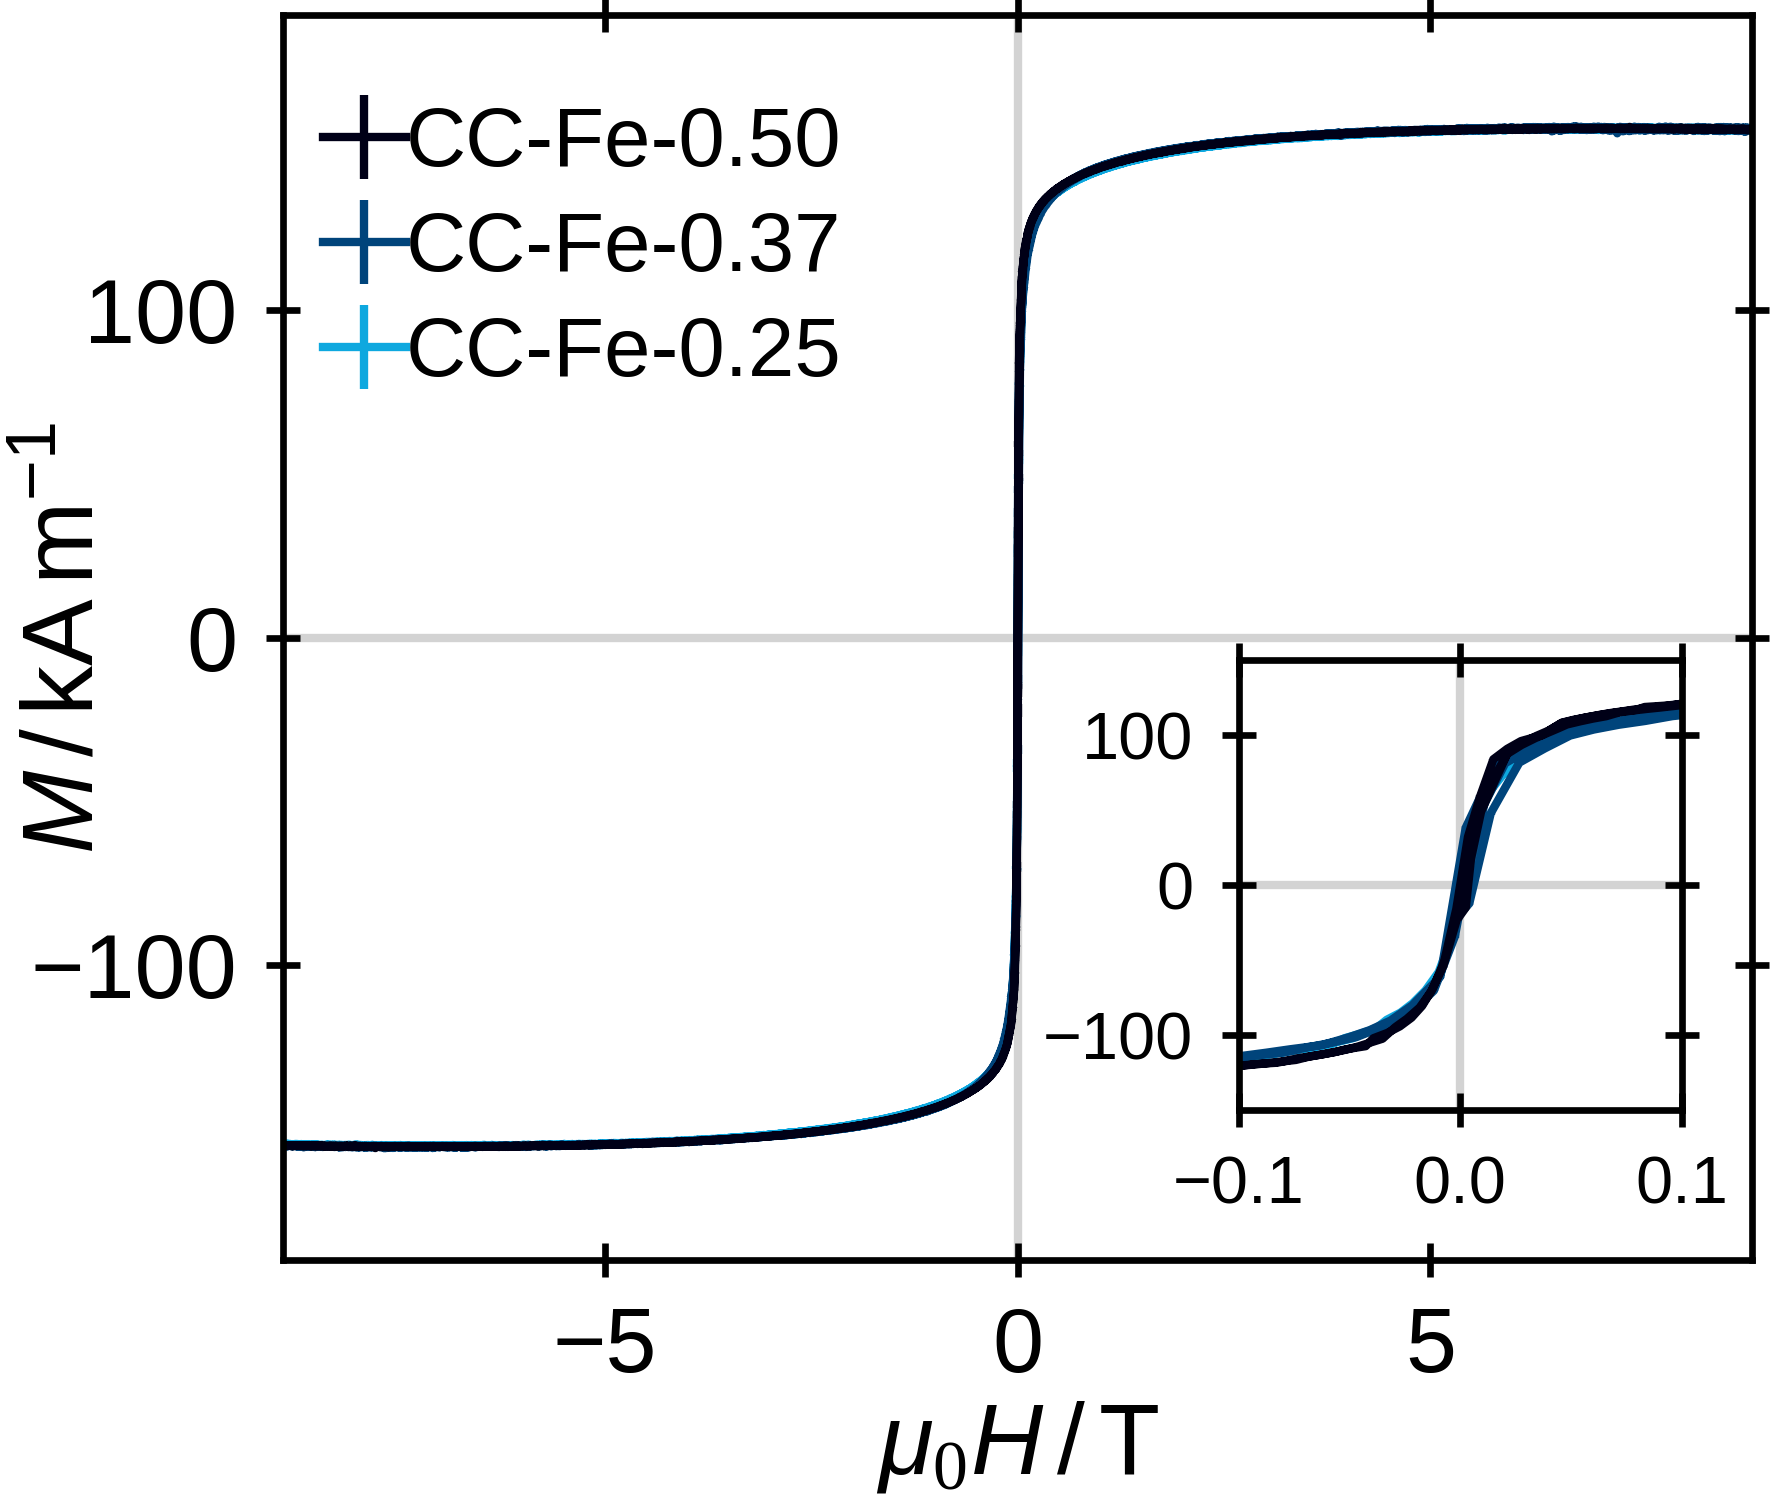
\includegraphics{colloidalCrystals_PPMS_300K_allSamples}
    \caption{\label{fig:colloidalCrystals:RTVSM}Field-dependent magnetization at $300 \unit{K}$ of the colloidal crystals. The as-measured data in units of $\mathrm{memu}$ (left) and the data corrected for the diamagnetic susceptibility of the background and scaled to the observed spontaneous magnetization as given in \reftab{tab:colloidalCrystals:RTVSM:parameters} (right).}
  \end{figure}

  To determine the macroscopic magnetization of the colloidal crystals, vibrating sample magnetometry experiments are performed on a PPMS Evercool II instrument (\refsec{ch:instruments:laboratoryInstruments:vsm}).
  By this macroscopic differences in the samples magnetization due to the varied layer thickness are investigated.

  \paragraphNewLine{Room temperature magnetization}
    In a first step the colloidal crystals are measured at room temperature to determine the spontaneous magnetization and susceptibility at high fields.
    By performing a linear fit between $5 - 9 \unit{T}$, the two values are obtained as tabulated in \reftab{tab:colloidalCrystals:RTVSM:parameters} and the fits in \reffig{fig:colloidalCrystals:RTVSM} (left).
%si density 2.32
    \begin{table}[!htbp]
      \centering
      \caption{\label{tab:colloidalCrystals:RTVSM:parameters} Spontaneous magnetization $M_s$ and excess susceptibility $\chi$ of the colloidal crystals determined by fitting the slope of the data in the range of $5 - 9 \unit{T}$. As well as scaled to the area of the silicon substrate.}
      \begin{tabular}{ l | l | l || l | l}
        \rule{0pt}{2ex} \textbf{VSM @ 300 K}
        & $M_s \, / \unit{memu}$
        & $\chi \, / \unit{\musf emu \, T ^{-1}}$
        & $\bar{M}_s \, / \unit{memu \, cm^{-2}}$
        & $\bar{\chi} \, / \unit{memu \, T ^{-1} cm^{-2}}$ \\
        \hline
        \rule{0pt}{2ex} CC-Fe-0.25    & $1.8480(4)$   & $-16.18(6)$ & $7.269(1)$   & $-0.0637(2)$\\
        \rule{0pt}{2ex} CC-Fe-0.37    & $1.5599(5)$   & $-5.46(7)$  & $10.748(4)$  & $-0.0376(5)$\\
        \rule{0pt}{2ex} CC-Fe-0.50    & $4.4333(7)$   & $6.68(9)$   & $15.237(2)$  & $0.0229(4)$\\
        \hline
      \end{tabular}
    \end{table}

    The observed values are scaled to the mass of the sample's silicon substrate and thereby the magnetizations are obtained as scaled with respect to the measured wafer surface.
    Dividing the scaled spontaneous magnetizations $\bar{M}_s$ of the three samples to the dispersion concentration used during sample preparation, approximately the same values of $29.08$, $29.05$ and $30.47$ in the units of $\mathrm{memu \, cm \, mg^{-1}}$ are obtained.
    Thereby, it can be seen that the measured spontaneous magnetization $\bar{M}_s$ is directly correlated to the used concentration of nanocubes in the sample preparation.
    The susceptibility of the curves is relatively small in direct comparison to the sample magnetization but tends to increase with the amount of nanocubes on the wafer.
    The observed susceptibility is a combination of the samples paramagnetism and the substrates diamagnetism, where for no paramagnetic contribution from the nanocubes a constant value across the three samples would be expected after scaling to the substrate mass.
    The variation shows that the nanocubes contribute possibly still due to a paramagnetic phase or spin disorder in the nanoparticles.

    Correcting the measured magnetization for the varying susceptibility and scaling the spontaneous magnetization to the value observed from the dry powder of nanocubes in \refsec{sec:colloidalCrystals:nanoparticle:vsm}, \reffig{fig:colloidalCrystals:RTVSM} shows that the three magnetization behaviors exactly match with one another.
    Thus, at large temperatures of $300 \unit{K}$ the magnetization behaviour is largely independent of the sample thickness.
    The samples are not described well by either a Langevin behaviour nor a combination of two Langevin behaviour as has been done in \refsec{sec:colloidalCrystals:nanoparticle:vsm}.
    This makes it difficult to estimate the magnetic moment from the magnetization data and thereby the measured sample volume needed for scaling the data to units of $\mathrm{kA \, m^{-1}}$.
    Therefore in the following the data is discussed in the following qualitatively as scaled to the spontaneous magnetization measured at $300 \unit{K}$.

  \paragraphNewLine{Temperature-dependent magnetization}
    \begin{figure}[tb]
      \centering
      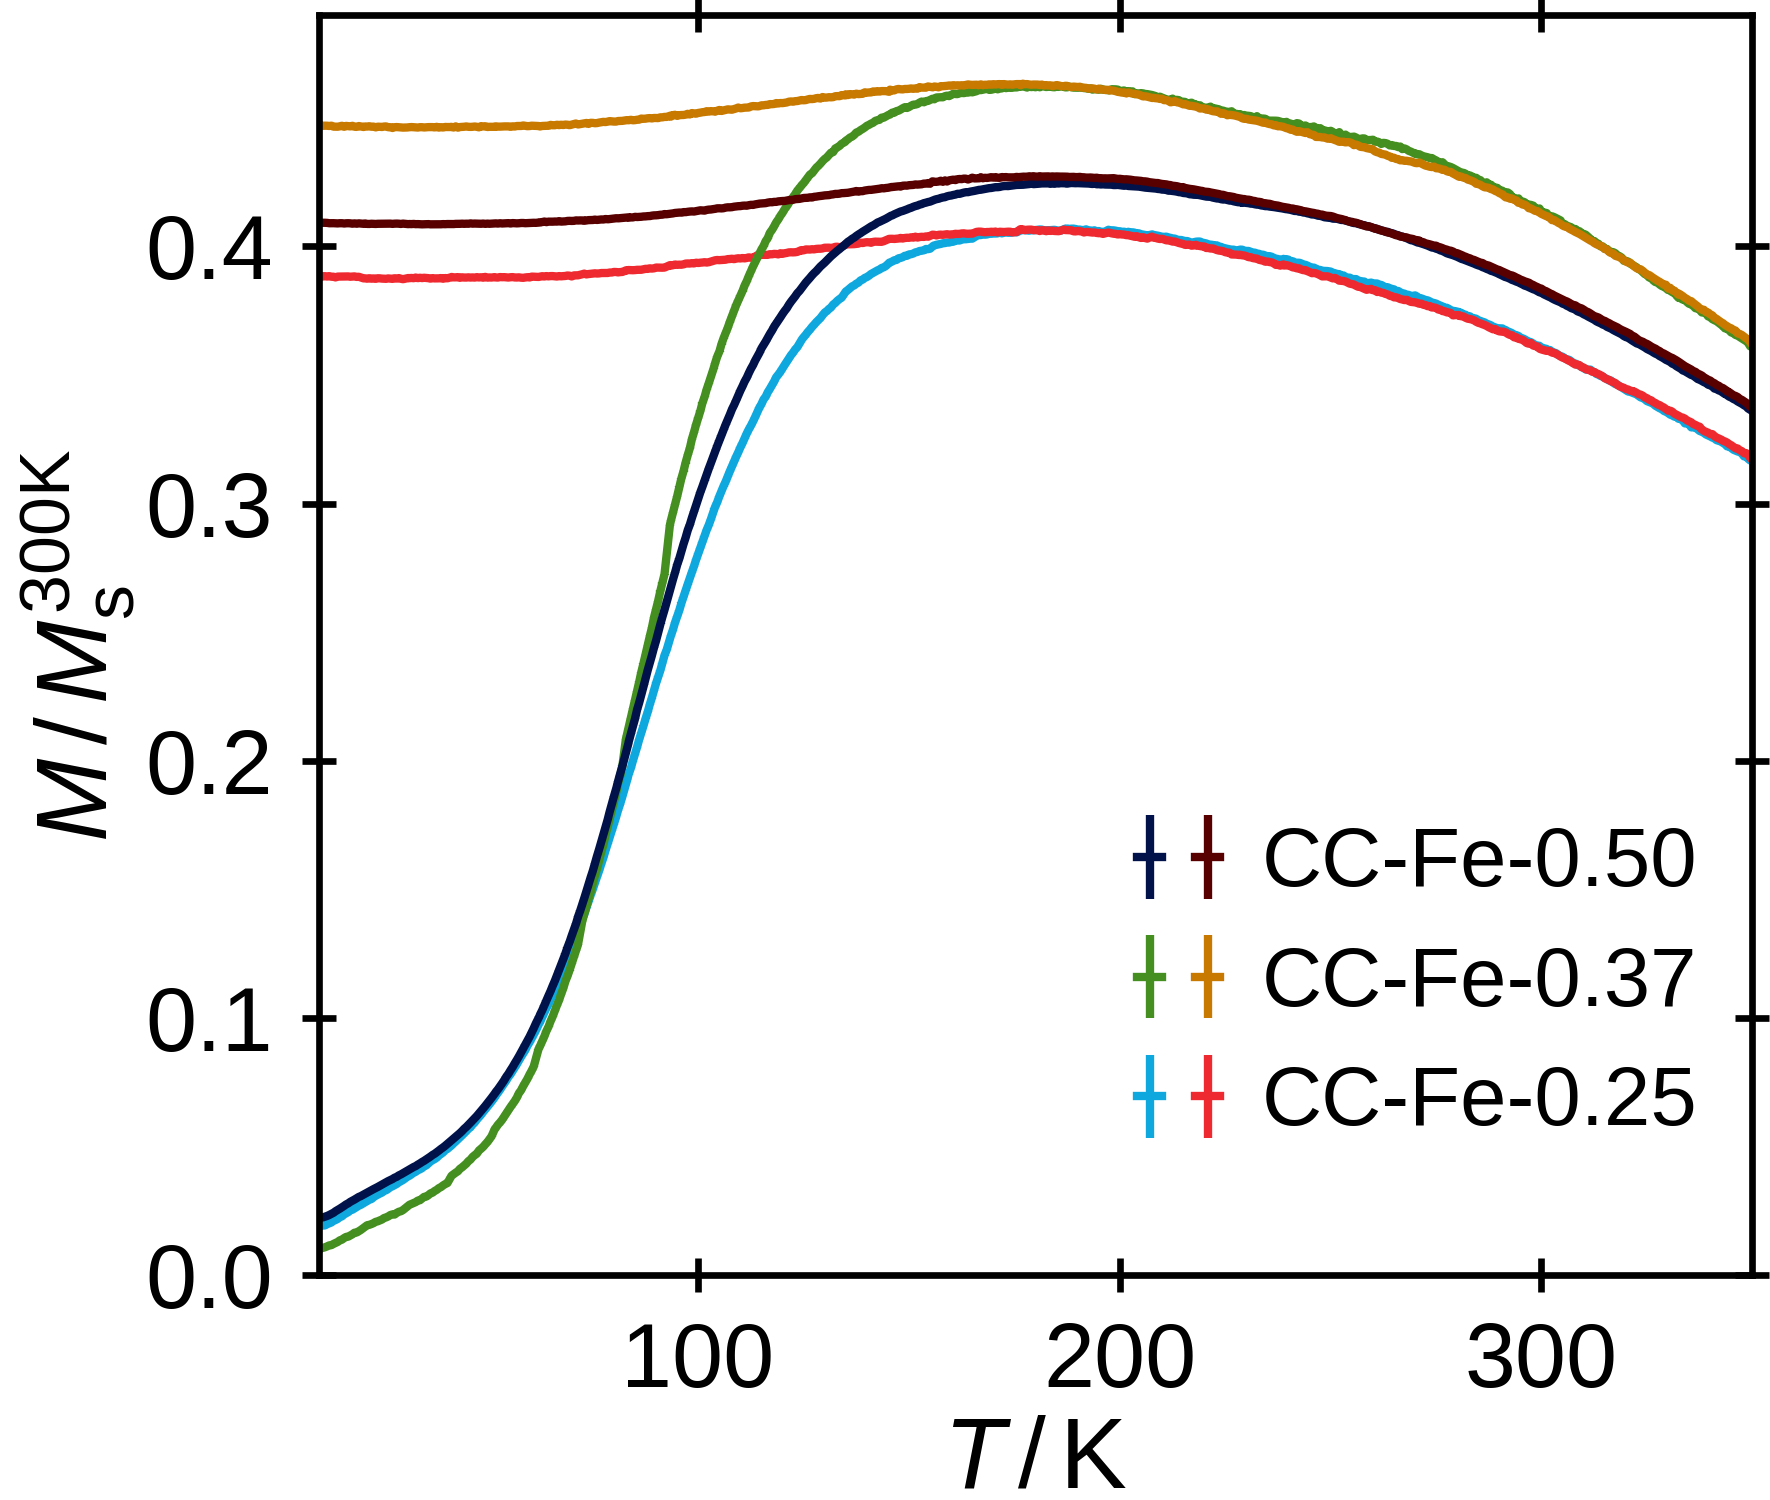
\includegraphics{colloidalCrystals_PPMS_ZFC_FC_allSamples}
      \caption{\label{fig:colloidalCrystals:zfcFCData}Zero-field cooled (red) and field cooled (blue) magnetizations of the three colloidal crystals. The ZFC/FC magnetization measurements are taken with a field of $10 \unit{mT}$ applied in the substrate plane while warming the sample.}
    \end{figure}

    \begin{table}[!htbp]
      \centering
      \caption{\label{tab:colloidalCrystals:ZFCFC:parameters} Temperatures of the peaks observed in the zero-field and field cooled magnetization of the colloidal crystals shown in \reffig{fig:colloidalCrystals:zfcFCData}.}
      \begin{tabular}{ l | l | l}
        \rule{0pt}{2ex} \textbf{ZFC/FC @ 10 mT}
        & $T_p^\mathrm{ZFCw} \, / \unit{K}$
        & $T_p^\mathrm{FCw} \, / \unit{K}$\\
        \hline
        \rule{0pt}{2ex} CC-Fe-0.25    & $188(1)$   & $182(1)$\\
        \rule{0pt}{2ex} CC-Fe-0.37    & $183(1)$   & $173(1)$\\
        \rule{0pt}{2ex} CC-Fe-0.50    & $188(1)$   & $183(1)$\\
        \hline
      \end{tabular}
    \end{table}

    For the colloidal crystals, the zero-field and field cooled magnetization is measured at a field of $10 \unit{mT}$ in the sample plane and shown in \reffig{fig:colloidalCrystals:zfcFCData}.
    The rescaling of the data was performed as determined from the spontaneous magnetization at room temperature.
    In each case a peak can be observed in both the field cooled and zero-field cooled curve, where the positions for the three samples is determined as tabulated in \reftab{tab:colloidalCrystals:ZFCFC:parameters}.
    It is visible that the temperatures of CC-Fe-0.37, are significantly shifted by $5 \unit{K}$ in the ZFC data and $9 \unit{K}$ in the FC data towards smaller temperatures than observed for CC-Fe-0.25 and CC-Fe-0.50, where the same peak values are observed.
    From SEM, the intermediate sample CC-Fe-0.37 was considered the sample with the best structural order among the three, which might show it's manifestation at this point.
    For dipolar interaction it is generally observed in literature that stronger dipolar interaction leads to an increase of the blocking temperature \cite{Morup_2010_Magne, Pauly_2012_Sized, Otero_2000_Influ}.
    Thus, in this manner the observation of a lower blocking temperature indicates weaker dipolar interaction within the sample CC-Fe-0.37 if the shift is associated with dipolar interparticle interaction.

  \paragraphNewLine{Field-dependent low temperature magnetization}

    \begin{figure}[tb]
      \centering
      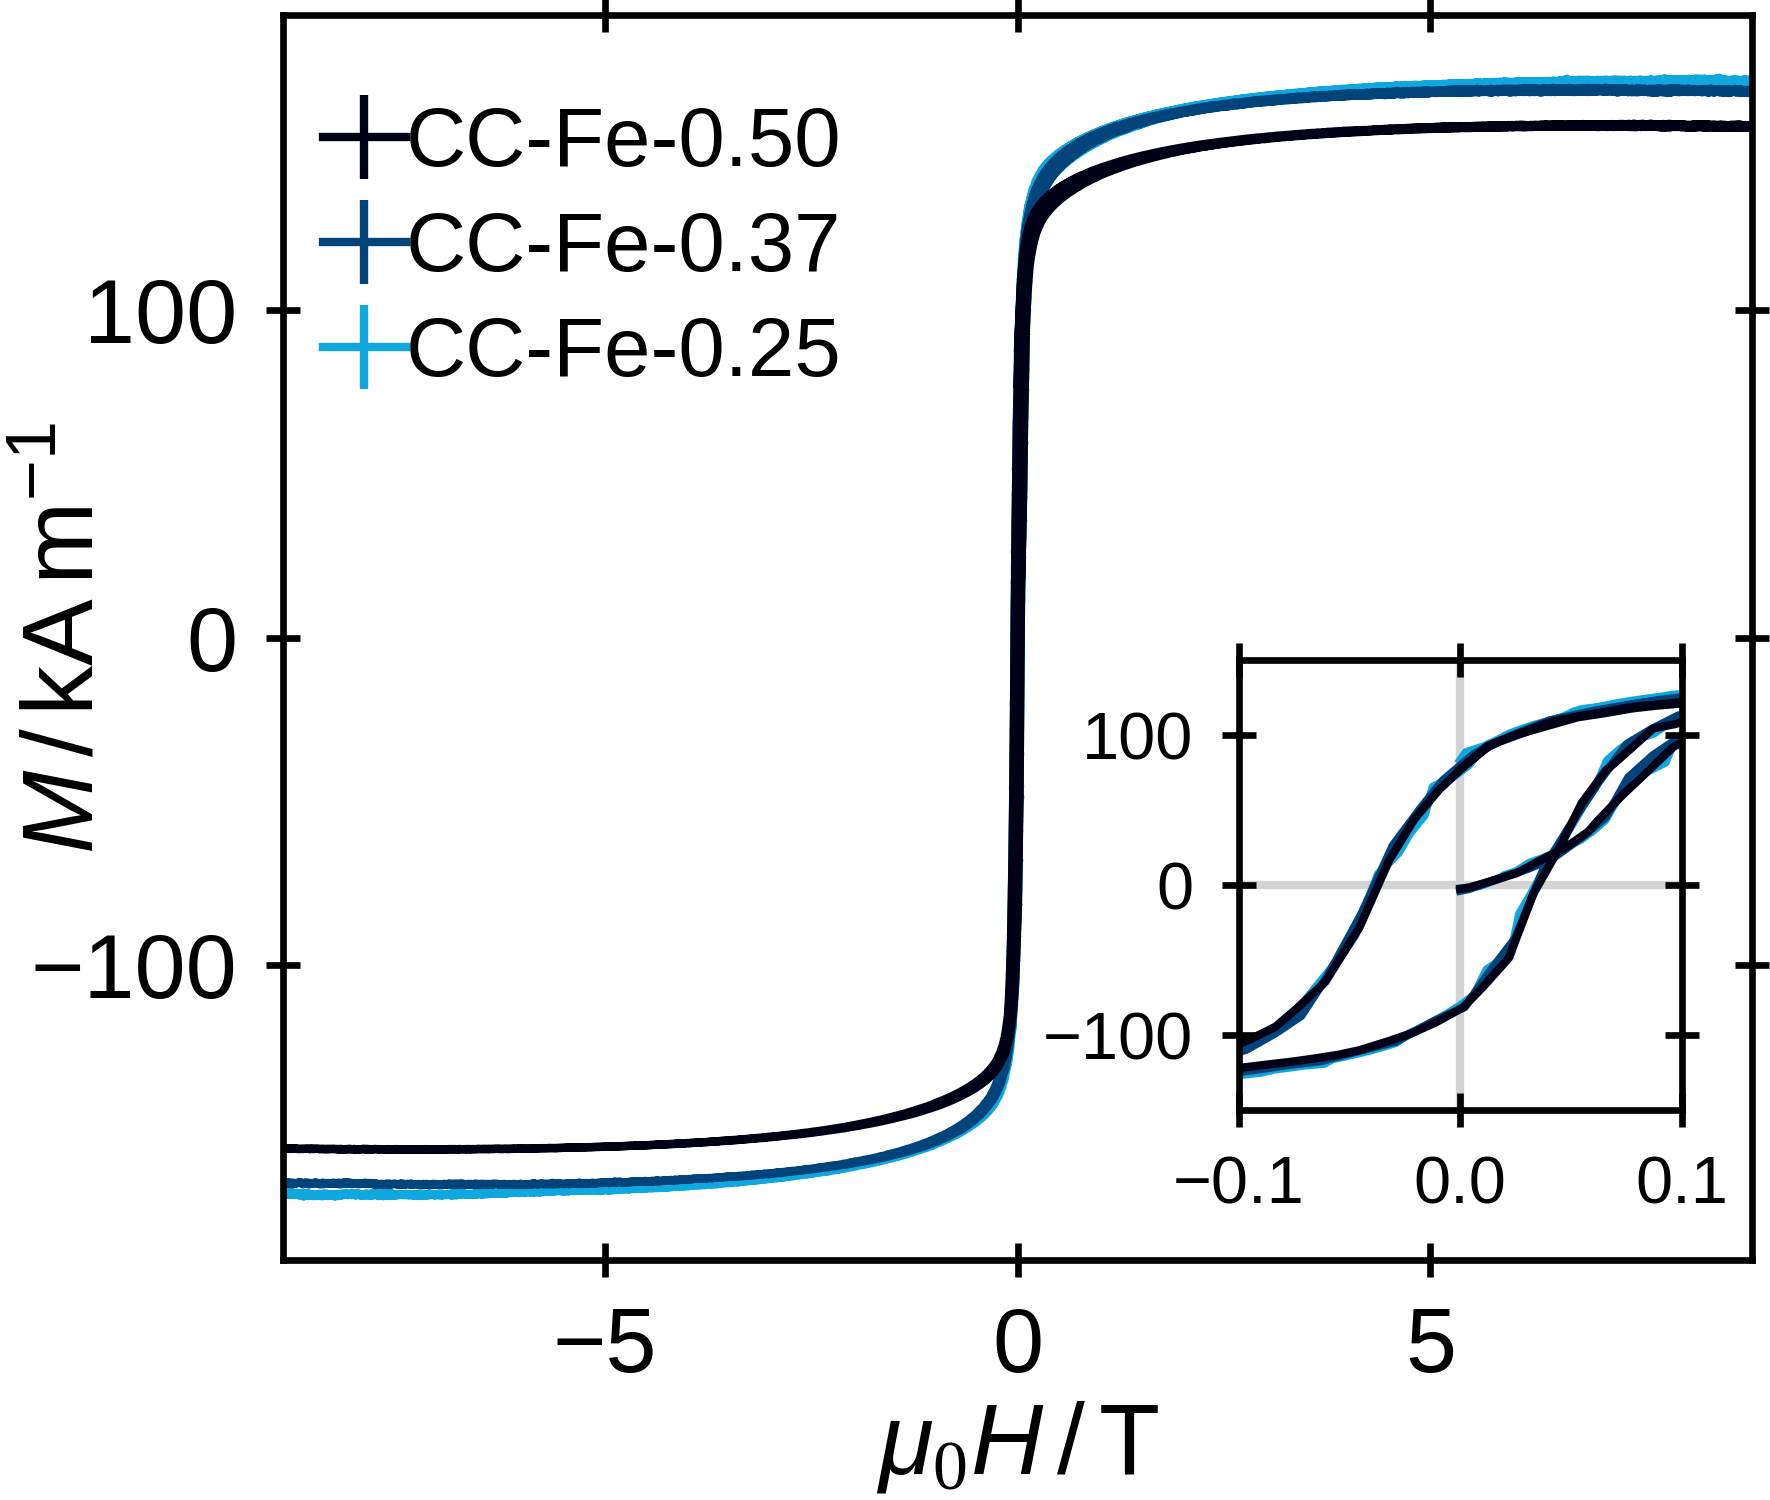
\includegraphics{colloidalCrystals_PPMS_10K_allSamples}
      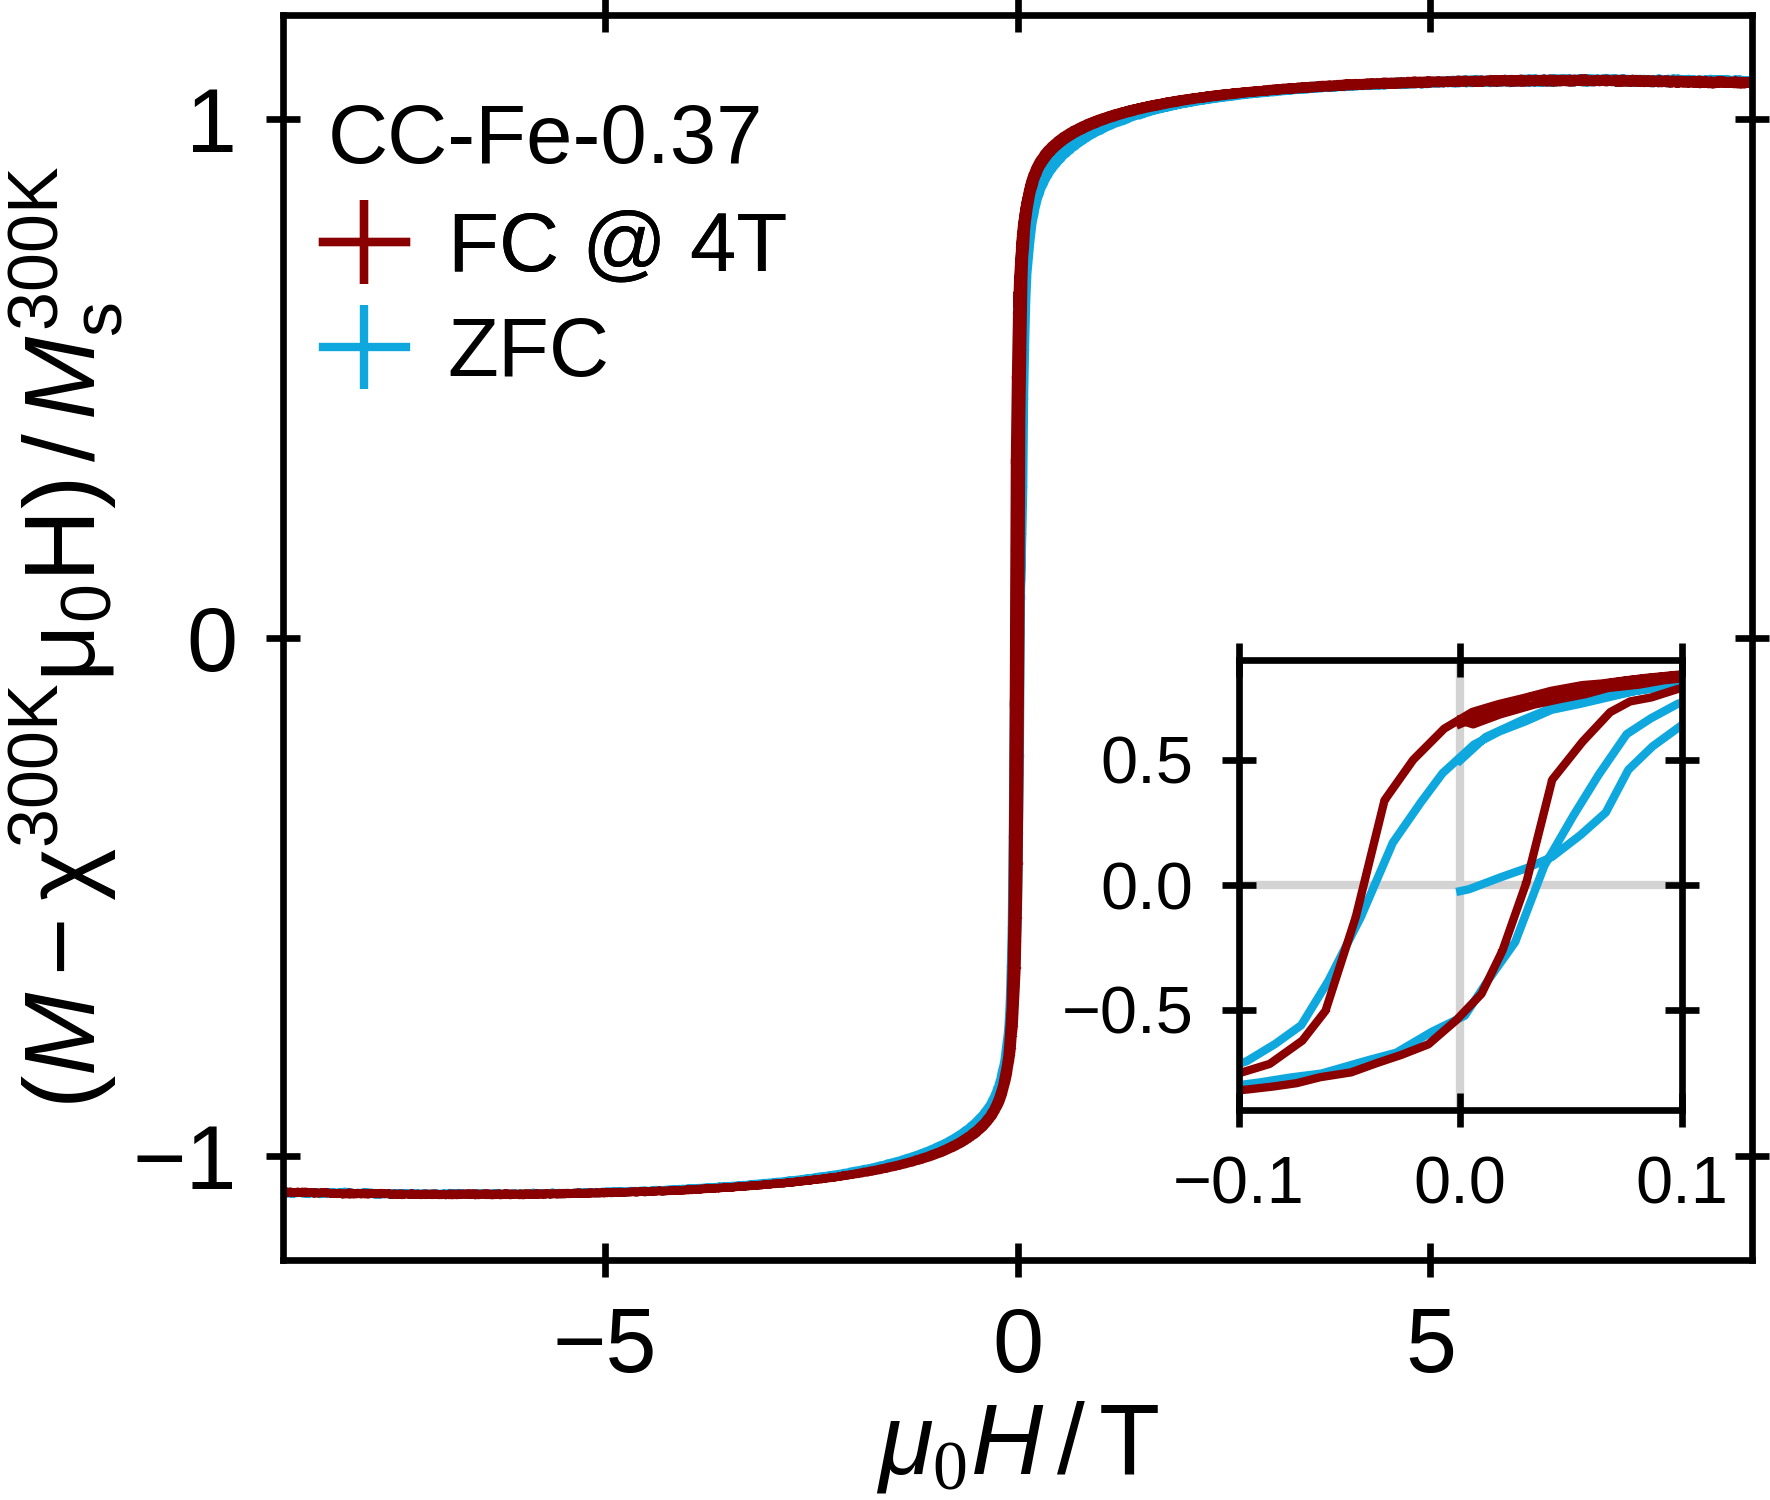
\includegraphics{colloidalCrystals_PPMS_10K_CC-Fe-0-37_EB}
      \caption{\label{fig:colloidalCrystals:10KVSM}Low temperature field-dependent magnetization of the colloidal crystals measured at $10 \unit{K}$. The colloidal crystals are all measured after zero-field cooling (left). Furthermore, the effect of field cooling the sample in a strong magnetic field of $4 \unit{T}$ on the hysteresis is shown for CC-Fe-0.37 (right).}
    \end{figure}
    The samples CC-Fe-0.25, CC-Fe-0.37 and CC-Fe-0.50 were both measured field-dependent at $10 \unit{K}$ after zero-field cooling. The data is rescaled as determined by the room temperature measurement and shown in \reffig{fig:colloidalCrystals:10KVSM}.
    It can be seen that at low magnetic fields, a close match in the coercive field is given, which is observed to be $35(1) \unit{mT}$.
    At larger fields the curves separate however and the thin sample CC-Fe-0.25 reaches a higher spontaneous magnetization in comparison to the thicker samples, where the lowest saturation value is observed for the CC-Fe-0.50 sample.
    Considering the strong magnetic fields that are applied to the sample, it is hard to imagine that this is an effect due to dipolar interaction within the sample at strong fields.
    It is probable that this splitting suggests a systematic error during the low-temperature measurement where possibly the sample shifted on the sample holder slightly on the sample holder during the measurement, which would not have been corrected by the touchdown procedure of the Evercool II instrument upon cool-down.

    Furthermore, it is studied which effect the application of a magnetic field during the cool down has on the example of the magnetization of CC-Fe-0.37.
    After cooling in a $4 \unit{T}$ field, a negative exchange-bias shift in the order of $5(1) \unit{mT}$ can be seen, as well as an increase of the remanent magnetization by $25 \%$.
    The saturating magnetization of the sample is otherwise analogue to the zero-field cooled hysteresis.
    As the magnetization measurements of the colloidal crystals have been measured $1 - 2$ years after the synthesis of the nanocubes and the preparation of the colloidal crystals it should be assumed that the iron oxide nanocubes have completely oxidized and no w\"ustite core is present in the sample.
    However, as discussed in \refsec{sec:colloidalCrystals:nanoparticle:xrd}, anti-phase boundaries should exist throughout the volume of the nanocubes and it is known in literature that these also induce an exchange-bias effect \cite{Wetterskog_2013_Anoma}.
    It is therefore probable that the observed shift of the hysteresis is a single-nanoparticle effect.
\end{document}